% include the figures path relative to the master file
\graphicspath{ {./content/method/figures/} {./content/intro/figures/} }

\section{Segmentation methodology description} 

Optimization methodologies offer a standardized manner to approach segmentation by minimizing an application-driven cost function~\cite{cremers2007review}.
\Cref{fig:method} illustrates a generic representation of the segmentation strategy here adopted to delineate breast tissues or lesions in \ac{us} images. 
The overall segmentation can be seen as a three-step strategy: 
(1) a mapping or encoding of the image into a discrete set of elements $\mathcal{S}$, 
(2) the optimization stage which is formulated as \emph{metric labelling} problem, 
and (3) re-mapping the labels obtained from the previous stage to produce the final delineation. 

\begin{figure}[htpb]
  \centering
  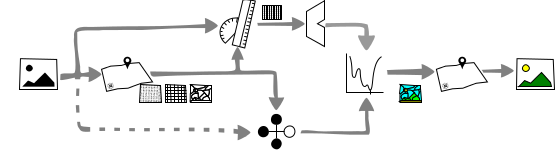
\includegraphics[width=0.9\linewidth]{method}
  \caption{Conceptual block representation of the segmentation methodology}
  \label{fig:method}
\end{figure}

In order to formulate the segmentation like a metric labelling problem, the image is conceived as a discrete set of elements $\mathcal{S}$ that need to be labelled using a label $l$ from the labelling set $\mathcal{L}$ 
(i.e.\, $l \in \{\text{lesion}, \overline{\text{lesion}}\}$ 
or $l \in \{\text{lungs}, \text{fat},\,\cdots\,, \text{lesion}\}$).
Let $\mathcal{W}$ be all the possible labelling configurations of the set $\mathcal{S}$, given $\mathcal{L}$.
Let $U(\cdot)$ be a cost function encoding the goodness of the labelling configuration $\omega \in \mathcal{W}$ based on the appearance of the elements in $\mathcal{S}$, their inner relation and some designing constraints.
Then, the desired segmentation $\hat{\omega}$ corresponds to the labelling configuration that minimize this cost function, as described in \cref{eq:costMin}.

\begin{equation}
\hat{\omega} = \arg \min_{\substack{\omega}} \,U(\omega)
\label{eq:costMin}
\end{equation}

The nature of $U(\cdot)$ and $\mathcal{W}$ determines which minimization strategies are applicable (or more desirable) in order to find $\hat{\omega}$; and which minimization strategies are not.

This goodness measure $U(\cdot)$ must be defined to take into account the appearance of the target region, its relation with other regions and other designing constrains.
\Cref{eq:labelingeq} describes this cost function as the combination of two independent costs that need to be simultaneously minimized as a whole.
The left hand side of the expression integrates the so called \emph{data} term, while the right hand side integrates the \emph{pairwise} term, which is also referred as the \emph{smoothing} term.
Both terms are shaped by $\mathcal{S}$ and evaluated in the labelling space $\mathcal{W}$.

\begin{equation}
  U(\omega) = \sum_{s\in s} D_s(\omega_s) + \sum_{s}\sum_{r \in \mathcal{N}_{s}} V_{s,r}(\omega_s,\omega_r)
  \label{eq:labelingeq}
\end{equation}

\Cref{fig:methodterms} illustrates the terms and elements relating the framework's outline, presented in \cref{fig:method}, with its formulation in \cref{eq:labelingeq}.
The problem of delineating the tissues present in \ac{bus} image has been used here for this illustrative purposes. 

\begin{figure}
    \centering
    \begin{subfigure}[b]{0.19\textwidth}
        \centering
        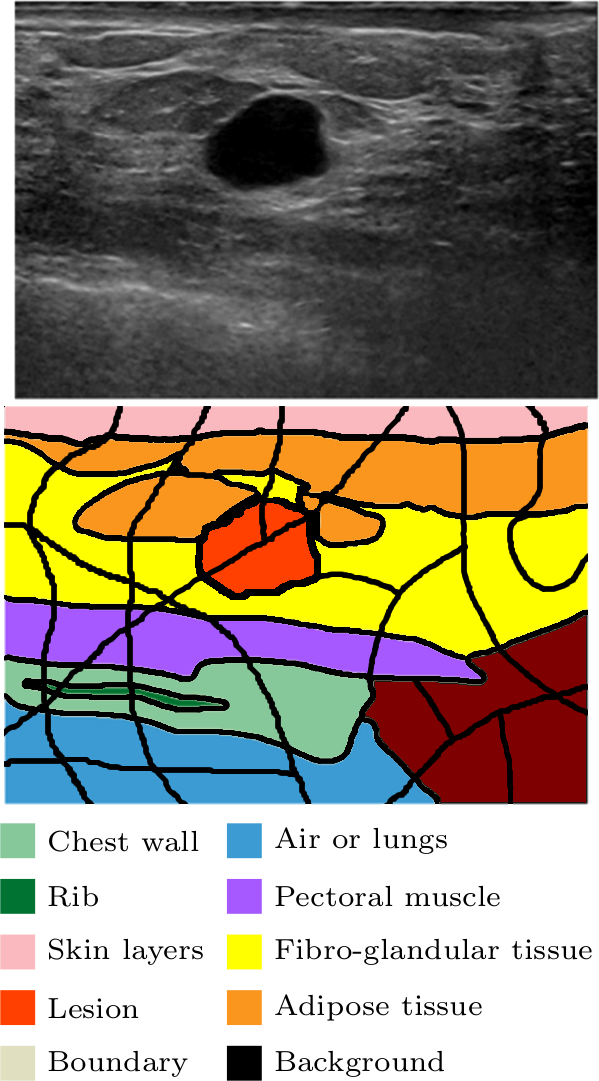
\includegraphics[width=\textwidth]{problem}
        \caption{{\small Problem definition}}    
        \label{fig:methodTerms:problem}
    \end{subfigure}
    \hfill
    \begin{subfigure}[b]{0.39\textwidth}  
        \centering 
        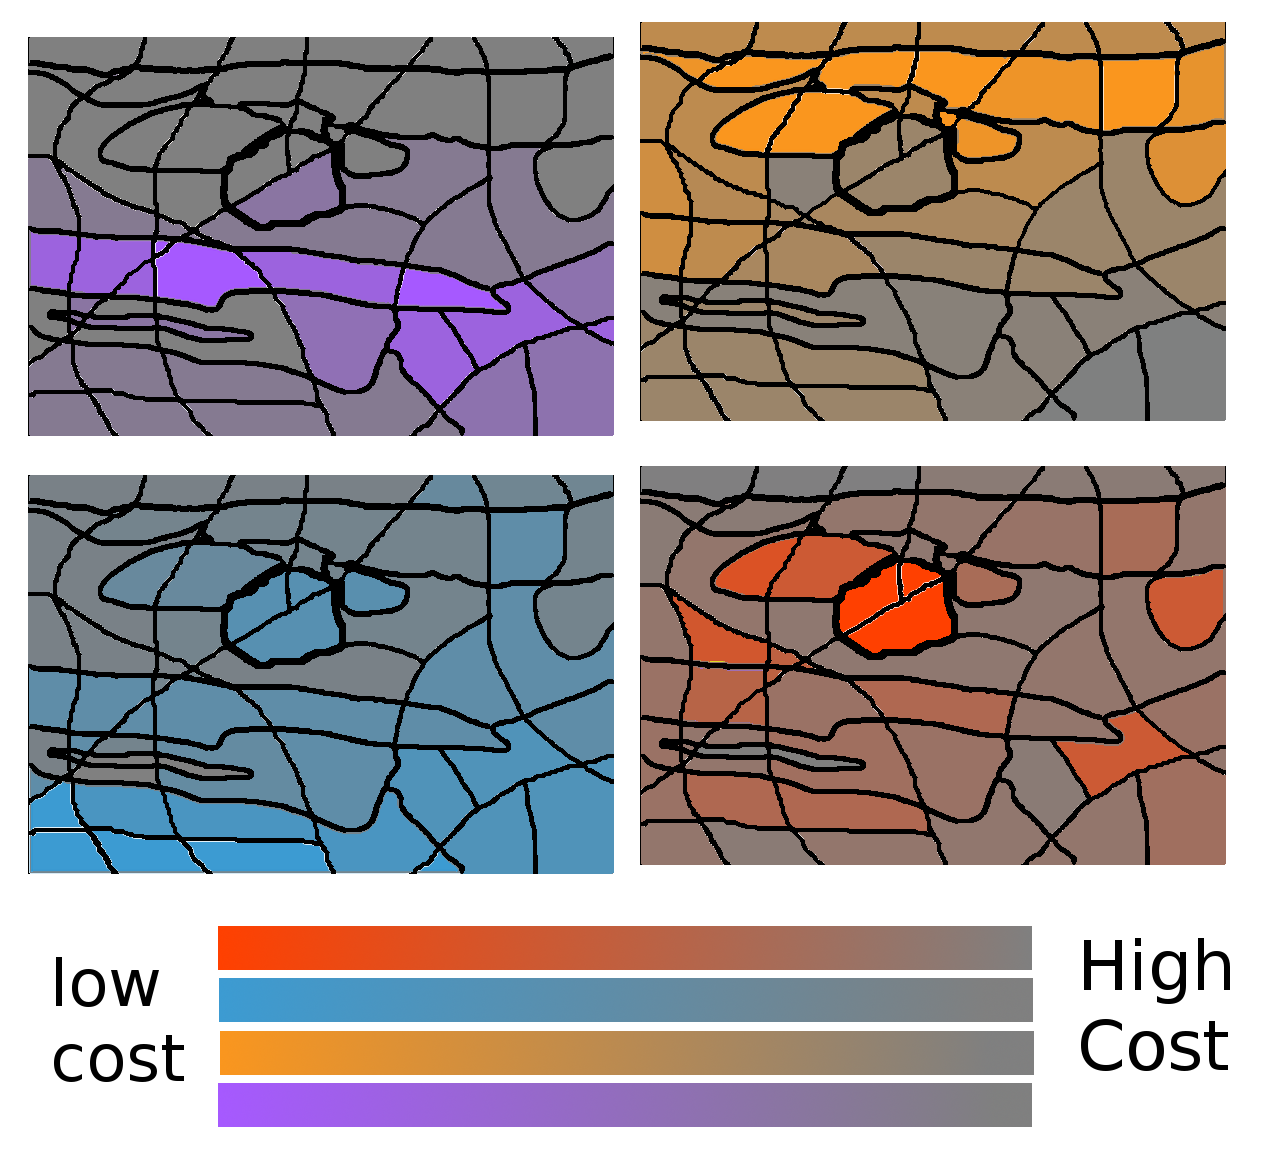
\includegraphics[width=\textwidth]{data}
        \caption[]%
        {{\small Data term}}    
        \label{fig:methodTerms:data}
    \end{subfigure}
    \hfill
    \begin{subfigure}[b]{0.39\textwidth}   
        \centering 
        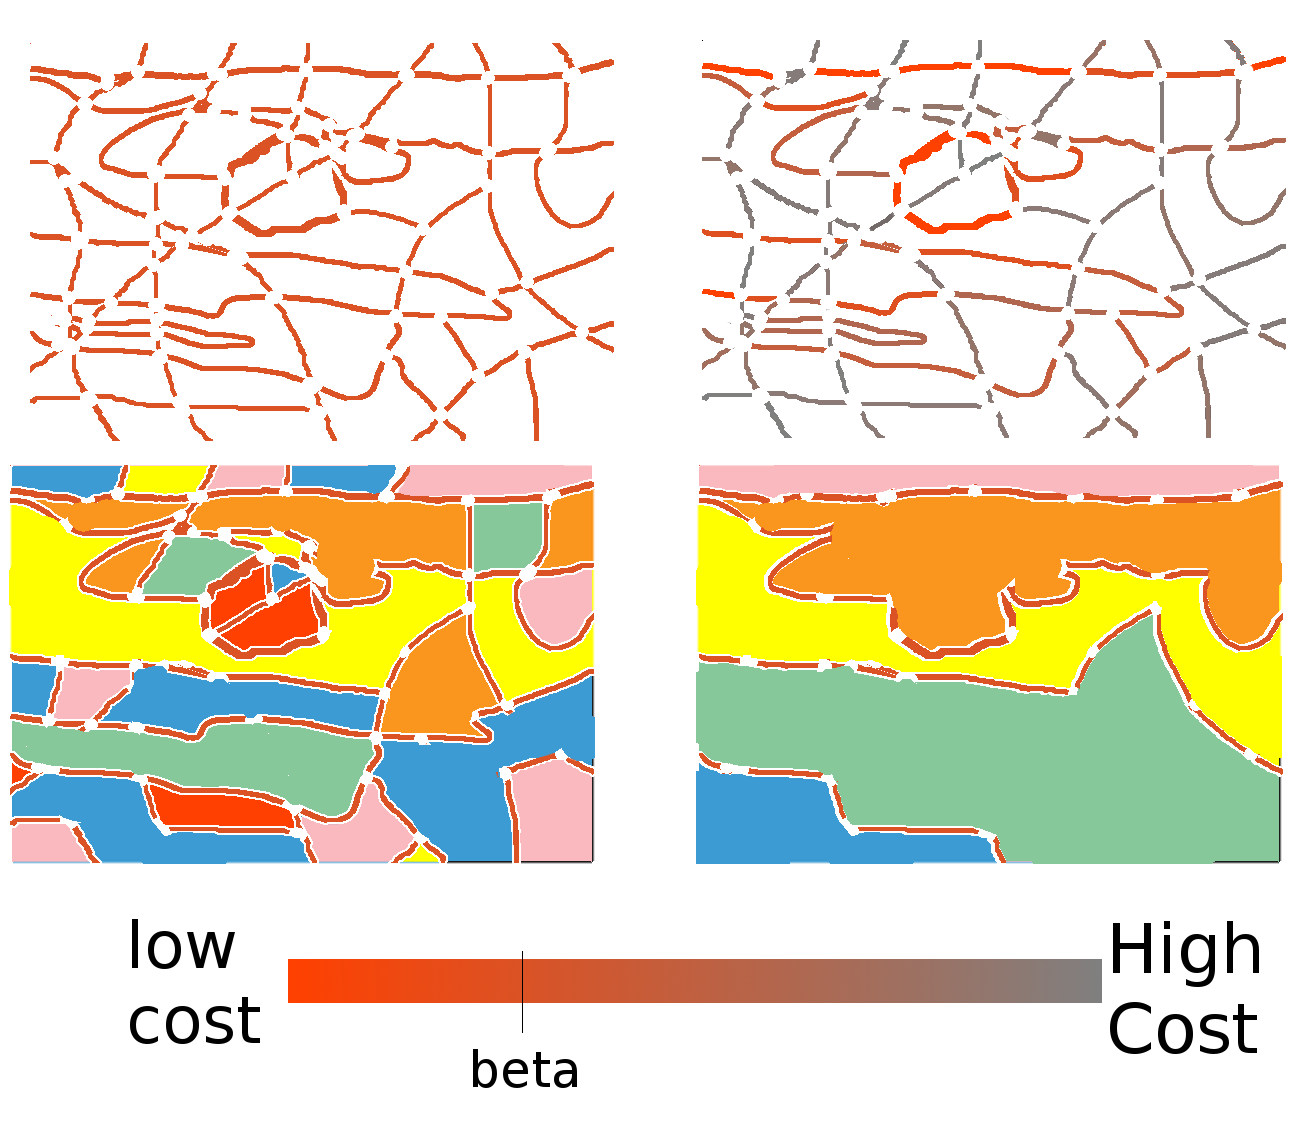
\includegraphics[width=\textwidth]{smooth} \caption[]%
        {{\small Pairwise term \emph{for this term the labels should be patterns and the cost be the only colour}}}    
        \label{fig:methodTerms:boundary}
    \end{subfigure}
    \caption {\small Methodology terms interpretation} 
    \label{fig:methodterms}
\end{figure}

In general, $\mathcal{S}$ can be any discrete set representing the image (i.e.\, pixels, overlapping or non overlapping windows, etc.). 
For this work $\mathcal{S}$ is chosen to be a super-pixels representation of the image.
Super-pixels can be seen as the output of a over-segmentation process or as a set of pixel collections that are contiguous and coherent with respect to some metric. Either way super-pixels are no overlapped irregular groups of similar connected pixels~\cite{achanta2012slic}.
\Cref{fig:methodTerms:problem} shows a \ac{bus} image example and a its associated super-pixels representation $\mathcal{S}$ coloured according to the image's \ac{gt}.

For the rest of this work, $\mathcal{S}$ is considered to be the super-pixels resulting from over-segmentation of the image using Quick-shift (see~\cite{massich2013phd} for details). 

Bear in mind that given an unseen \ac{bus} image, the ultimate goal is to represent the image as a set of super-pixels and infer the appropriated labelling for each of them.
To do so using the strategy here proposed, it requires to define: a data term, a pairwise term, and a proper minimization methodology.

\subsection{Data term} \label{sec:method:dataTerm}

Given a label configuration $\omega \in \mathcal{W}$, the data term penalizes the 
labelling of a particular image element or site ($\omega_s = l$) based on the data associated to $s$. 
In this manner $D_s(\omega_s=l_\cmark) << D_s(\omega_s=l_\xmark)$. 
\cref{fig:methodTerms:data} shows some labelling configurations $\omega'$ where all the sites share the same label, $\omega' \in \{ \omega_s=l,~\forall s\in\mathcal{S}\}$ to illustrate the effect (or behaviour) of this data term.
On it, the labelling preference of each site based on its appearance can be easily observed when comparing this labelling configurations.

Designing an obscure heuristic to comply with the desired behaviour of $D(\cdot)$ out of the box, is rather a complicated task.
Therefore, an easier and cleaner approach is to take advantage of \ac{ml} techniques to design this data cost in a systematic manner based on a training stage. 
The idea is to generate a data model for each class from training samples, and let $D(\cdot)$ be a distance or goodness measure reflecting the likelihood for $s$ to to belong to class $l$.
Defining the data term in this manner allows for great flexibility while offering a systematic approach towards its design.  
Using \ac{ml} to define $D(\cdot)$ allows for customizing the features to represent the data, allows for customizing the construction of the model where several classifiers and training techniques can be applied; or even to include some arbitrary constrains.

Despite regarding the construction $D(\cdot)$ are out of the scope of this report, the rest of this~\cref{sec:method:dataTerm} summarizes the process.
For further details the reader is referred to Massich et al.~\cite{massich2013phd}.
The usage of \ac{ml} as part of the proposed framework to determine $D(\cdot)$ is represented at the upper side of the diagram in~\cref{fig:method},
where two main blocks allow for design: 
(a) the features to represent the samples,
and (b) the tools to encode $D(\cdot)$ based on the features and the training. 

\subsubsection{\ac{bus} features to build the data term}
\Cref{fig:features:lexicon} illustrates the \ac{birads} lexicon: a standardized description of the visual cues found in \ac{bus} images, widely used by radiologists to produce a diagnosis based on the image readings. 

\Cref{fig:features} relates the \ac{birads} lexicon and the features designed to build $D(\cdot)$.

The following features are extracted to describe the sample $s$:
\begin{description}
  \item[Appearance] 
    Based on the multi-labelled \ac{gt}, a \ac{mad} histogram model for every tissue label is build. The Appearance feature is computed as the \ac{qc} distance between histogram of $s$ and the models.
  \item[Atlas] 
    Based on the multi-labelled \ac{gt} an atlas is build to encode the label likelihood based on the location of $s$.
  \item[Brightness] 
    Takes an intensity descriptor of $s$ (\emph{i.e:} mean, median, mode) and compares it with some intensity markers of the set $\mathcal{S}$ such as the minimum intensity value, the maximum, its mean, etc.
  \item[\ac{sift}-\ac{bof}]
    $s$ is represented as the occurrences of a \ac{sift} dictionary of 36 words~\cite{massich2014sift}.
\end{description}

In order to incorporate multi-resolution, each super-pixel is group with its adjacent super-pixels such that $s' = \{s \cup \mathcal{N}_{s}\}$, the features are recalculated using $s'$ and concatenated to the original feature descriptor. This operation can be repeated several times.

\emph{Mass shape}, \emph{Mass orientation}, and \emph{Mass margin} are in not encoded in $D(\cdot)$ since this visual cues do not belong to a single super-pixel but to the group of contiguous super-pixels sharing the same label. 
Otherwise lesions and super-pixels should be elements of same order.
This is not the case since the bottom-line is to label small regions to from the segmentation.
For similar reasons, the \emph{Lesion boundary} cue has been left out of the data term.
In order to take the echogenic halo into account as a super-pixel appearance, those should be small enough to be contained within the halo limiting the high-level region description allowed by larger super-pixels.


\begin{figure}
    \centering
    \begin{subfigure}[b]{0.28\textwidth}
        \centering
        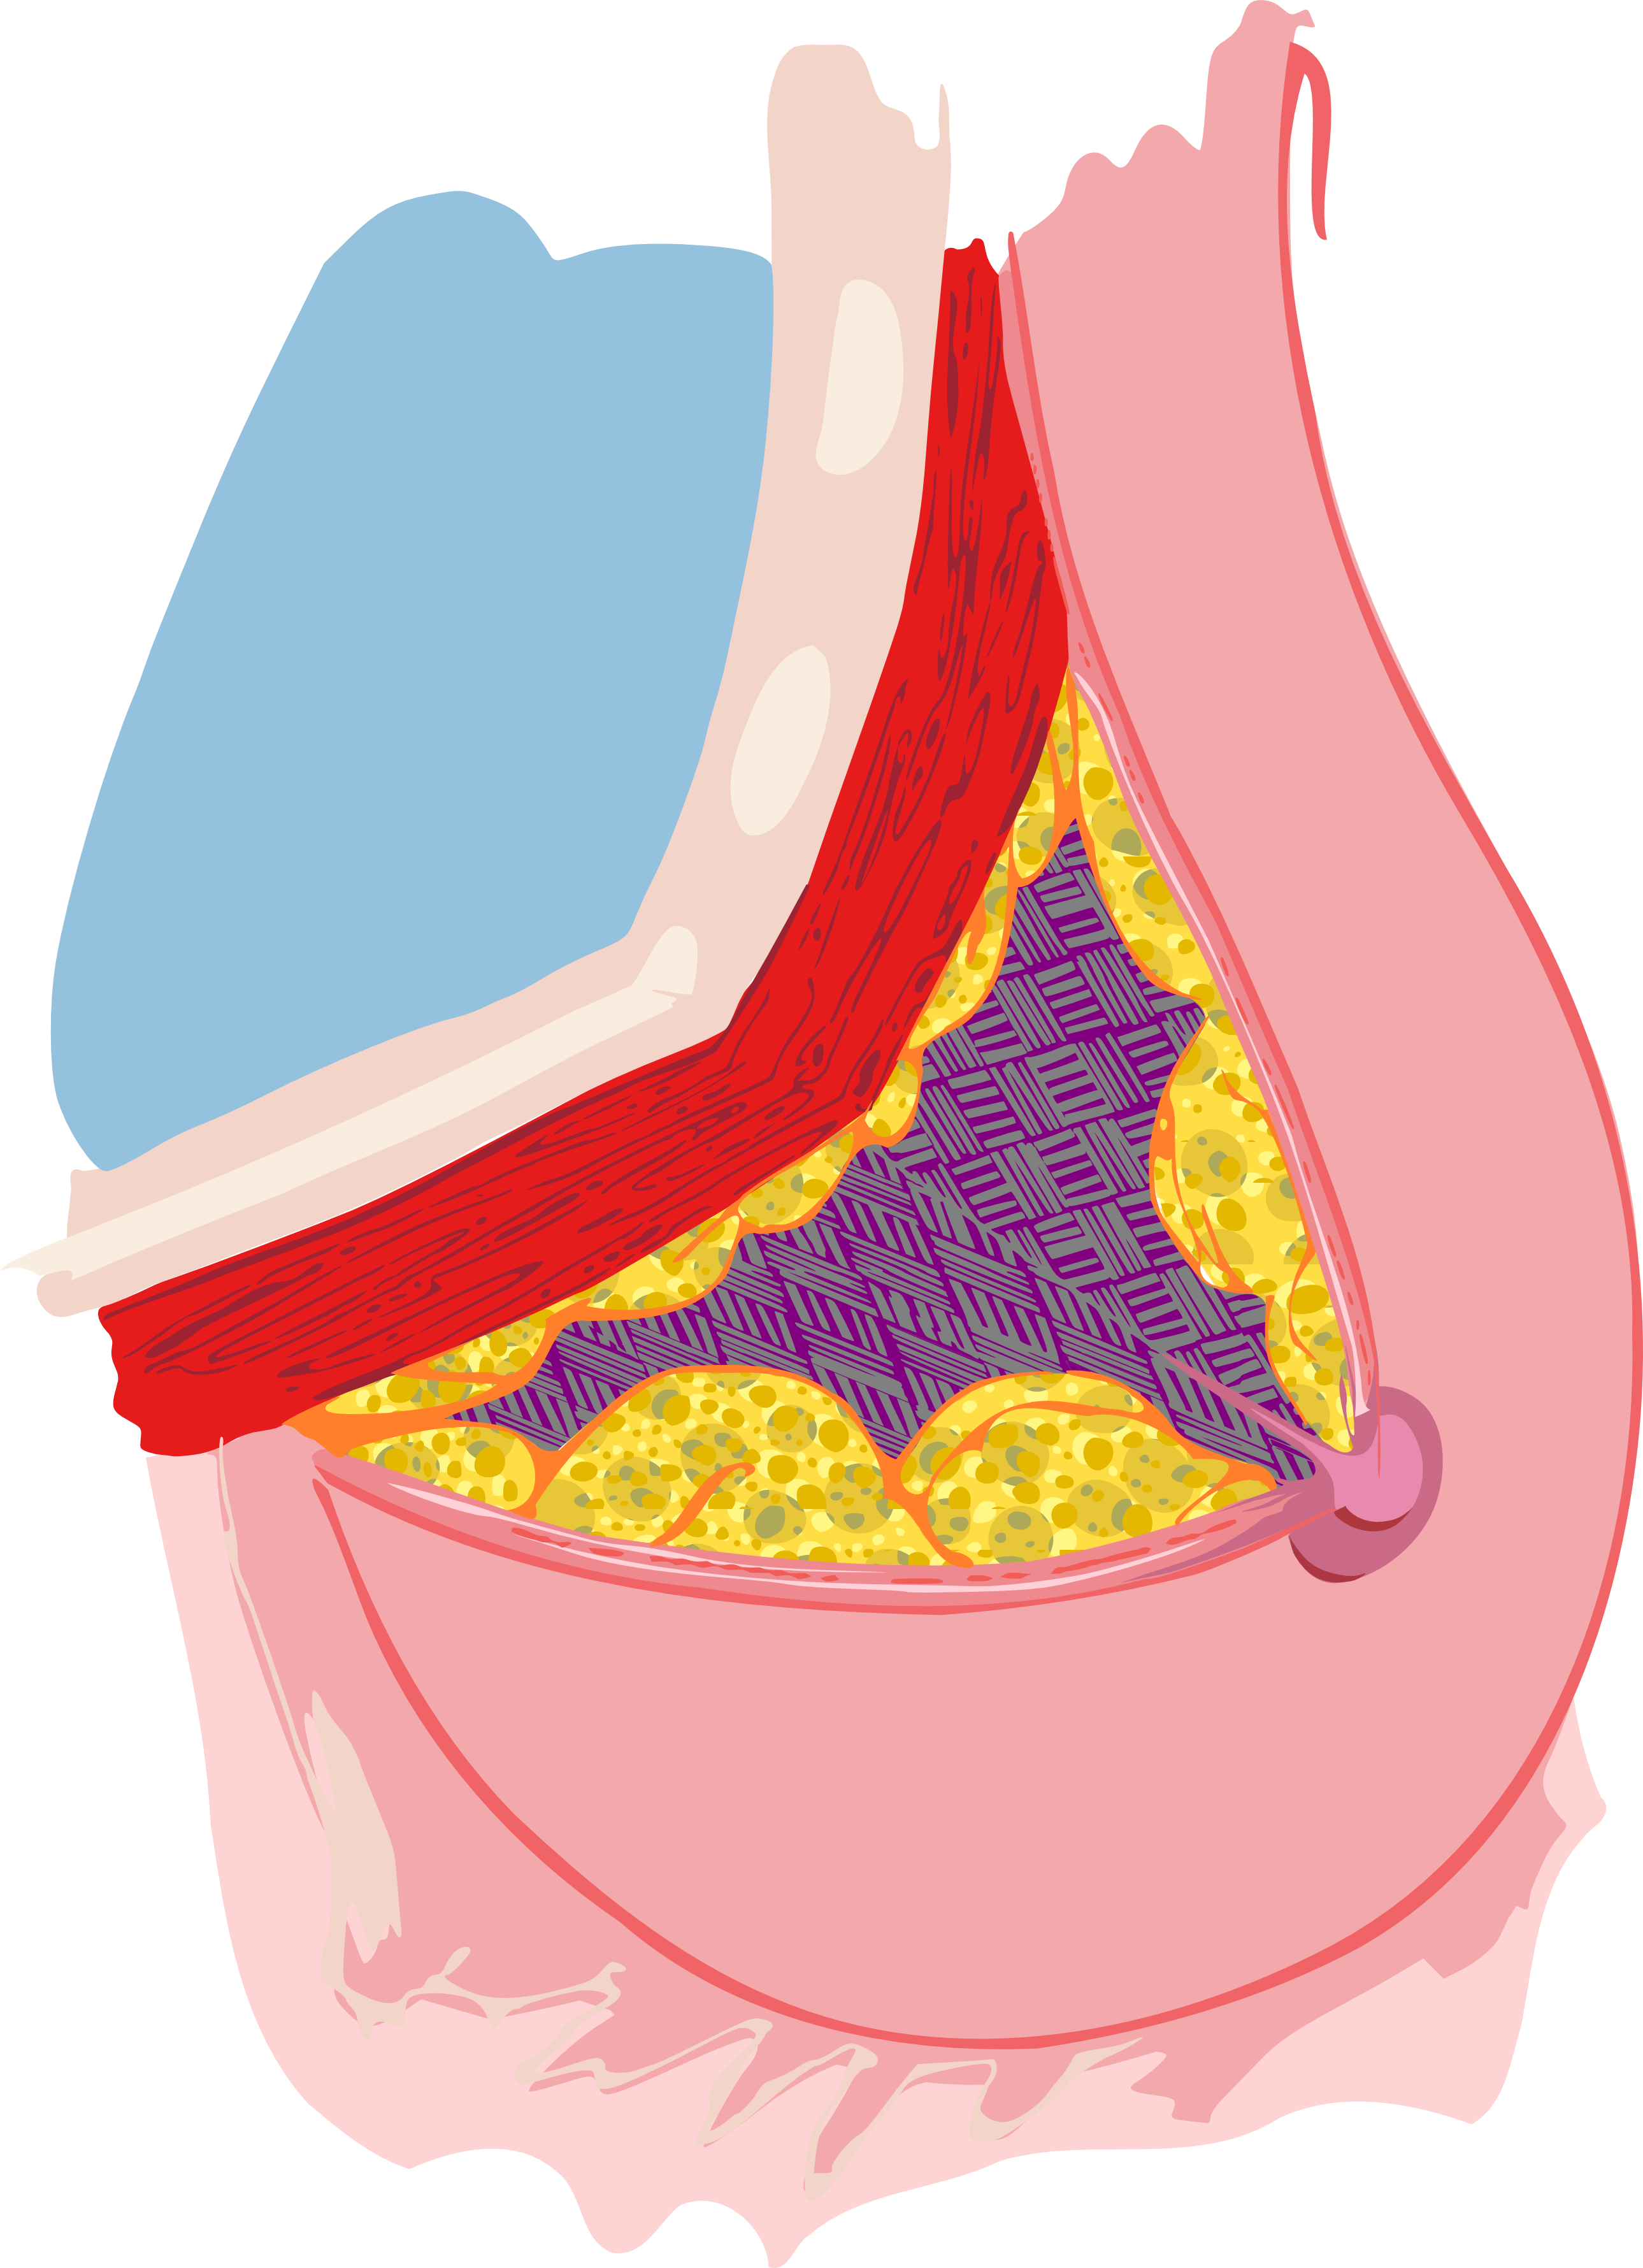
\includegraphics[width=0.5\textwidth]{breast}
        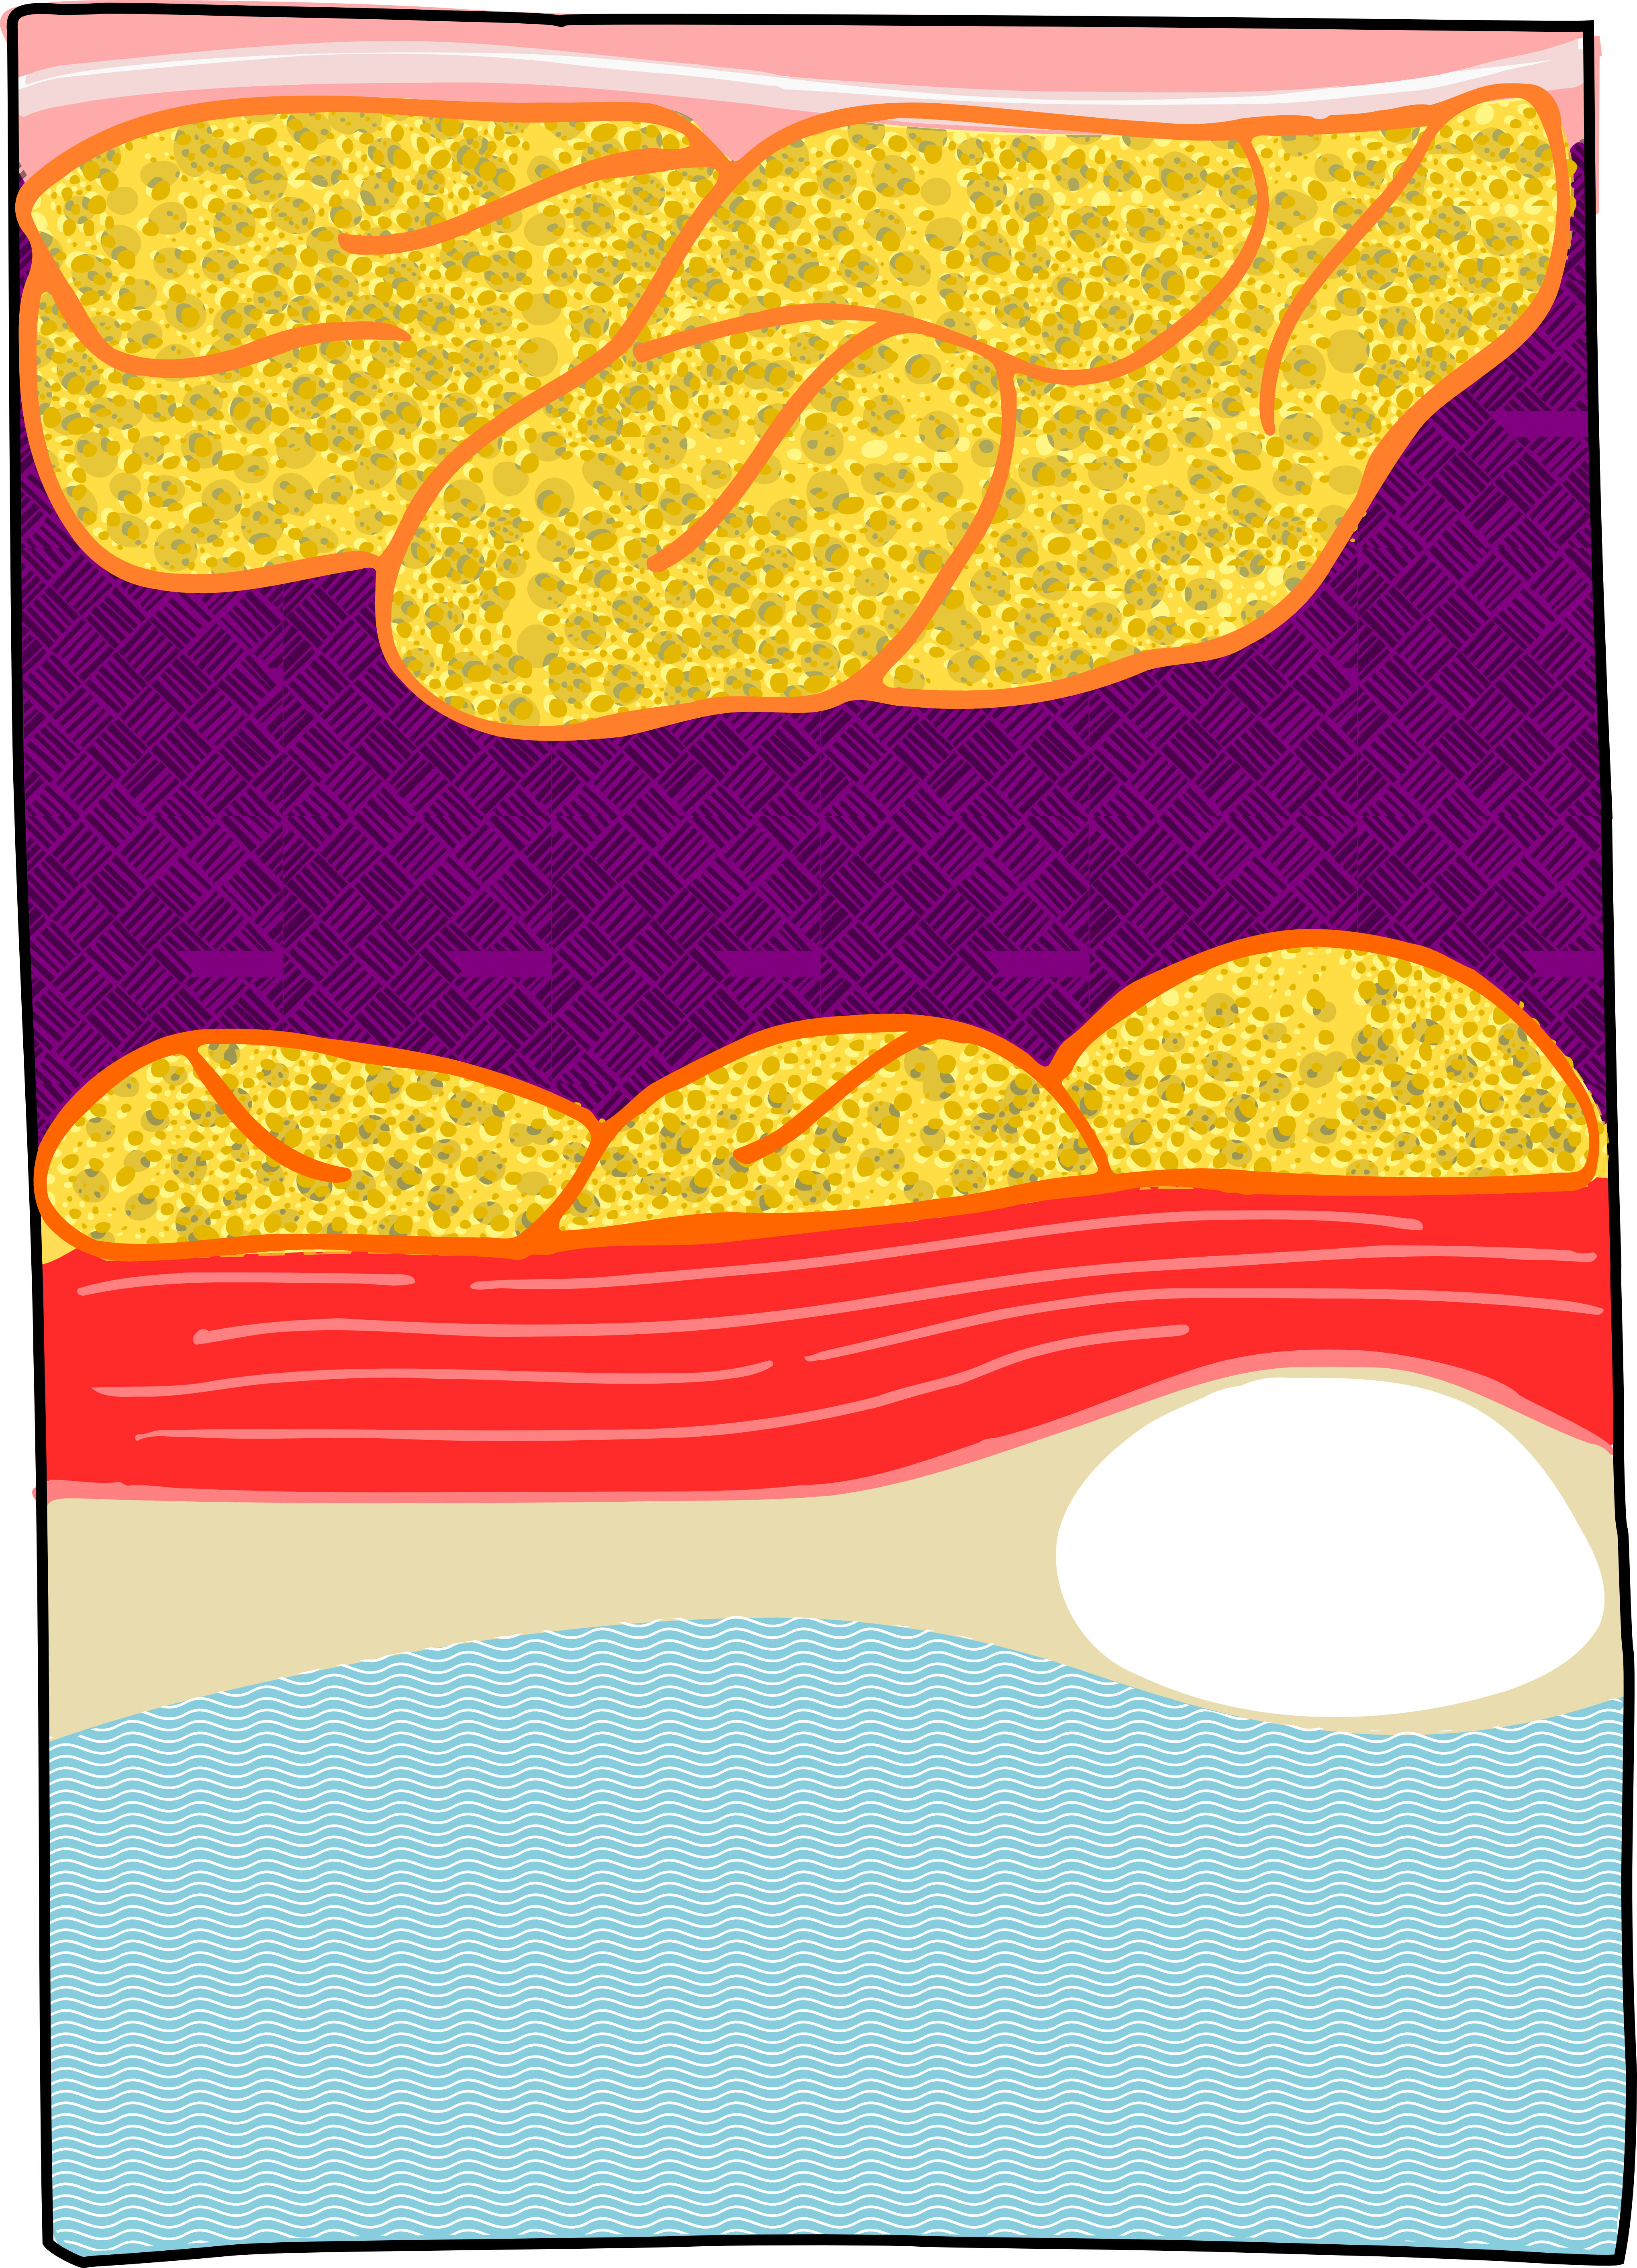
\includegraphics[width=0.5\textwidth]{slice}
        \caption{{\small Breast structure}}    
        \label{fig:features:breast}
    \end{subfigure}
    \hfill
    \begin{subfigure}[b]{0.4\textwidth}   
        \centering 
        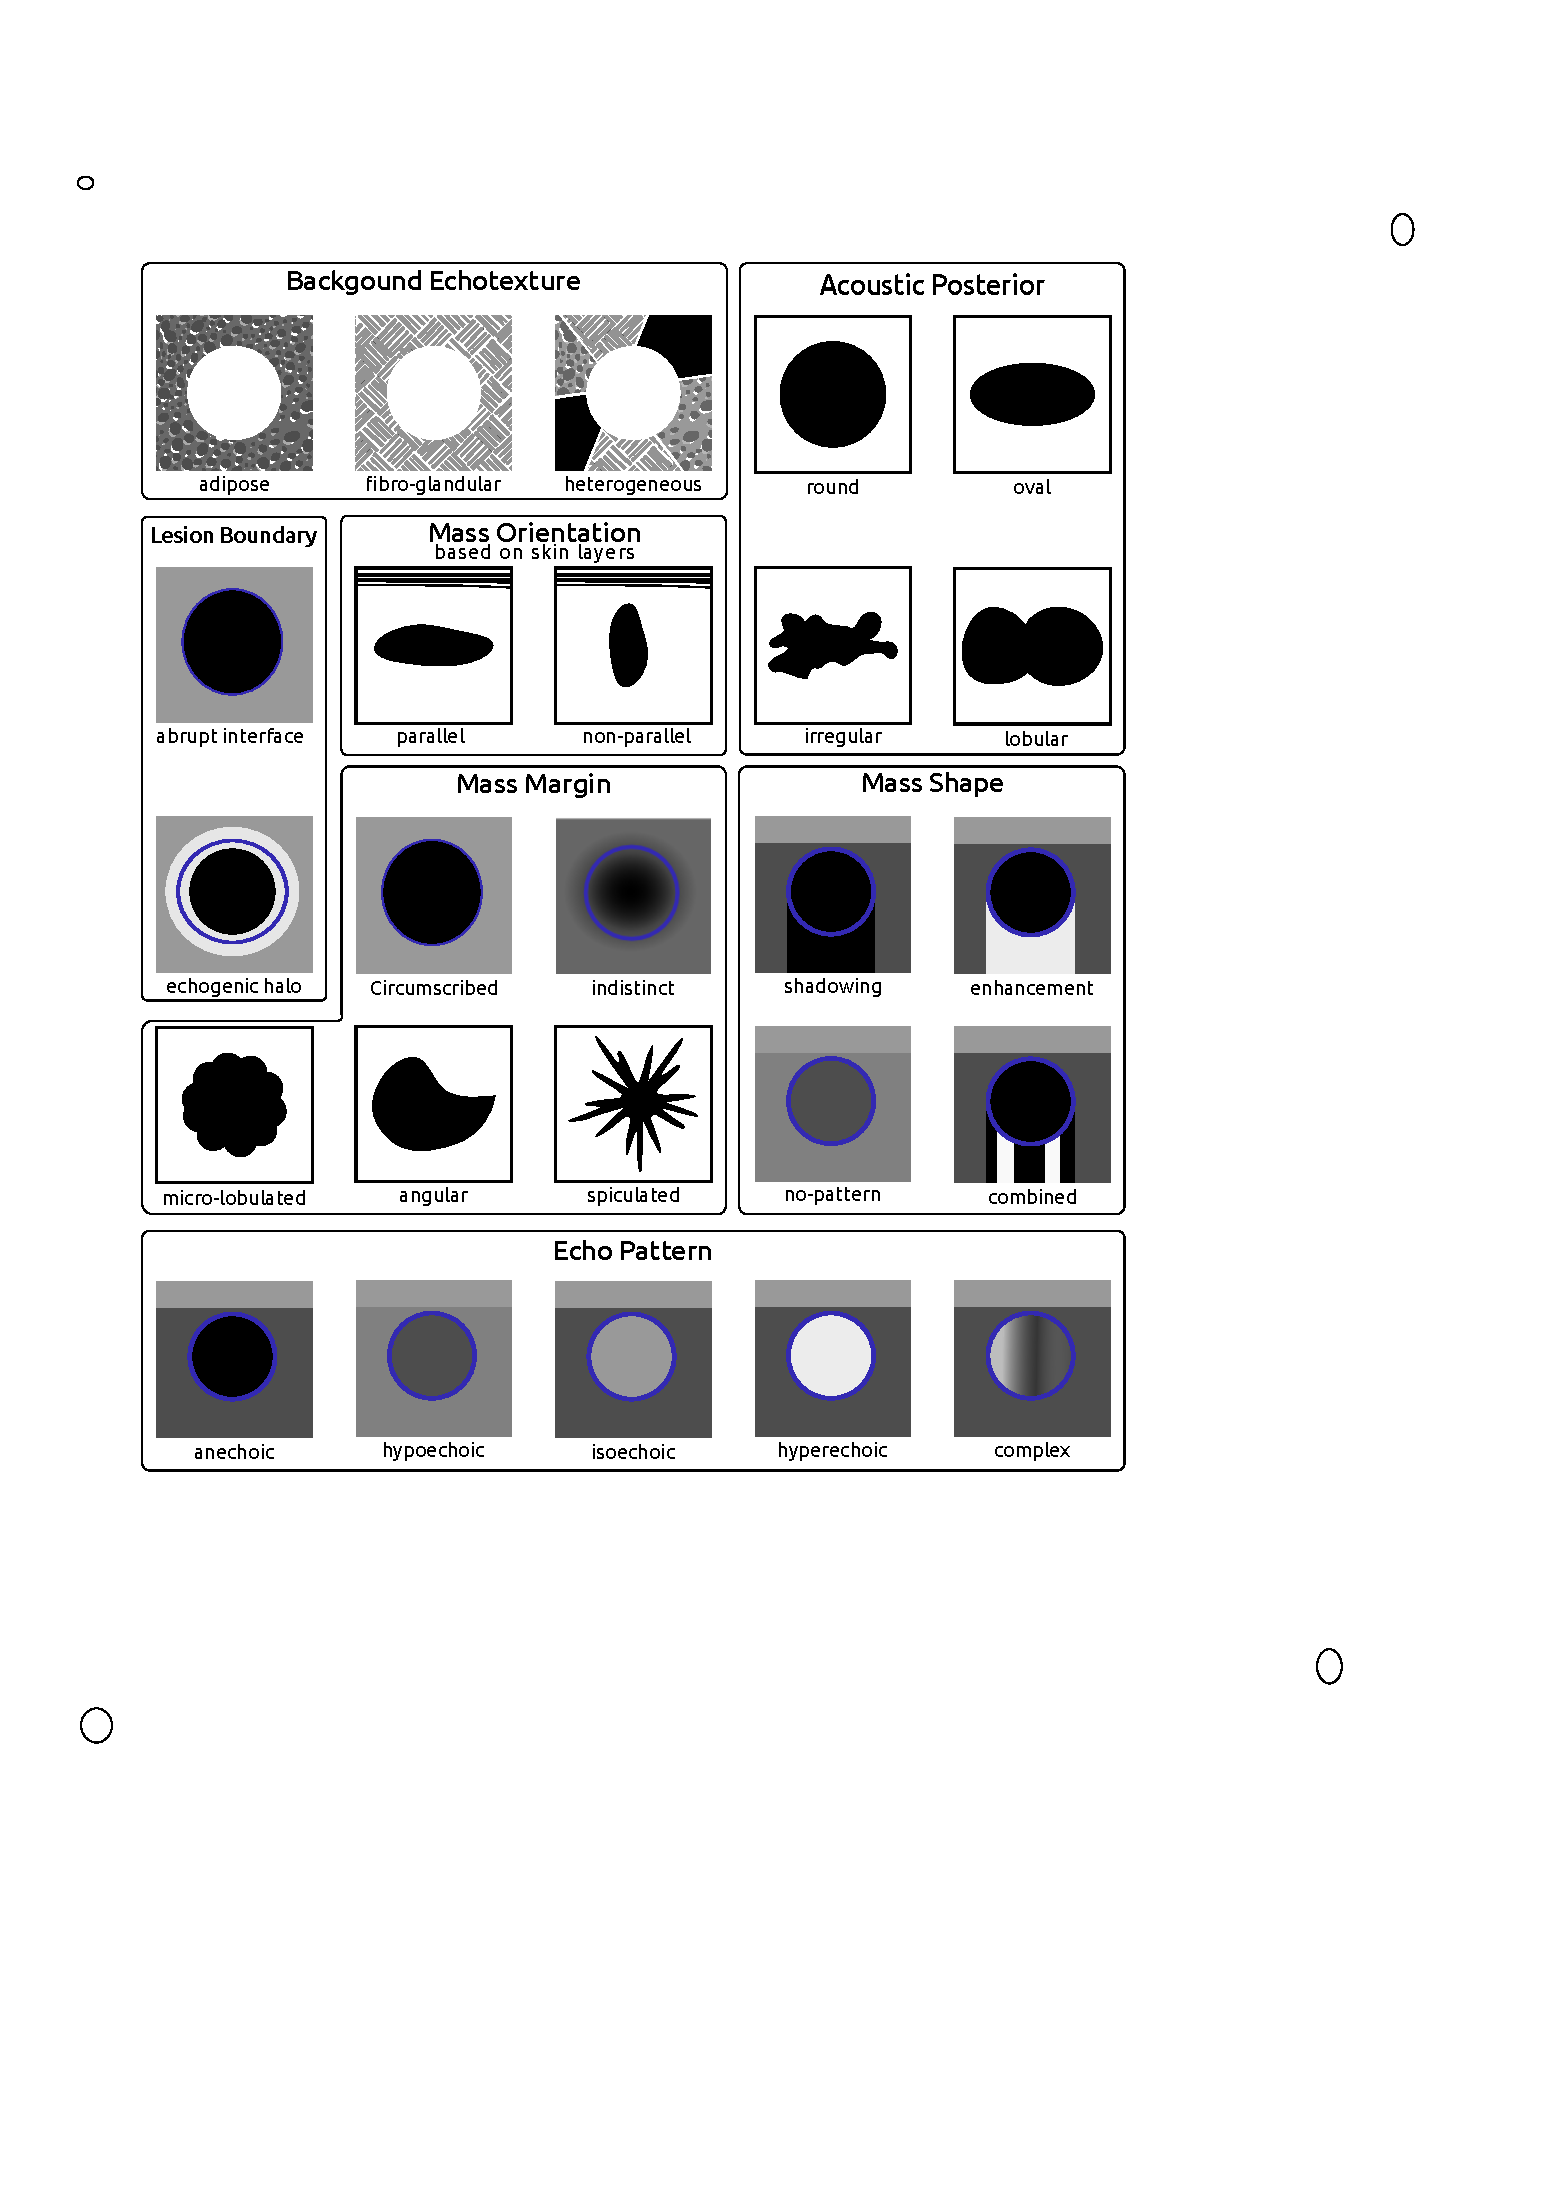
\includegraphics[trim = 65 345 200 124, clip,width=\textwidth]{birads}
        \caption[]%
        {Breast lesion characteristics in \ac{us} screening influencing clinical management~\cite{raza2010us}}    
        \label{fig:features:lexicon}
    \end{subfigure}
    \\
    \begin{subfigure}[b]{\textwidth}
      \centering
      \begin{tabular}{lcccccccc}
                  &Background Echo-Texture  
                  &Posterior  %Acoustic Posterior
                  &L.Boundary %Lesion Boundary
                  &M.Orient.  %Mass Orientation        
                  &M.Margin   %Mass Margin      
                  &M.Shape    %Mass Shape      
                  &E.Pattern\\%Echo Pattern\\
       Appearance & x &   &  &  &  &  & x & \\
       Atlas      &   & x &  &  &  &  & x & \\
       Brightness &   & x &  &  &  &  & x & \\
       SIFT-BoF   & x &   &  &  &  &  &   & \\
      \end{tabular}
    \end{subfigure}
    \caption {{\small Visual reference of breast structures and visual cues used for standard \ac{bus} image assessment and diagnosis.}} 
    \label{fig:features}
\end{figure}


\subsection{Pairwise or smoothing term} \label{sec:method:mrfTerm}
 
The pairwise term represents the cost of the assignation $\omega_s$ taking into account the labels of its neighbour sites, $\omega_r$, $r \in \mathcal{N}_{s}$. 
This term models a \ac{mrf} or a \ac{crf}.
The typical form of this term, given in \cref{eq:smoothing}, is called homogenization which acts as a regularization factor favouring configurations that have coherent labelling.

\begin{equation}
V_{s,r}(\omega_s,\omega_r) = 
\begin{cases}
    \beta, & \text{if } \omega_s \ne \omega_r\\
    0,              & \text{otherwise}
\end{cases}
\label{eq:smoothing}
\end{equation}

\Cref{fig:methodTerms:boundary} offers a visual interpretation of this cost.
If the resulting segmentation associated to the current labelling configuration $\omega$ has a boundary segment, this boundary brings a penalization $\beta$ to the total cost $U(\omega)$.
In this manner the regularization term can be seen as a post-processing or denoising stage since some sites will flip their labelling if the cost of producing and edge is larger than the cost of adopting the neighbour's label. 

More sophisticated smoothing terms where boundaries have different penalization based not only on site relations in $\mathcal{S}$ but also based on image information would (see \cref{fig:methodTerms:boundary}) be found in the final version of the manuscript.% in \cref{sec:smoothing}.

% Review %contribute have different or variable costs (see \cref{fig:methodTerms:boundary}) are also possible by taking into account not only relations in $\mathcal{S}$ of but also image information (see \cref{fig:method}). 
%Further details can be found in \cref{sec:smoothing}.

\subsection{Searching the best labelling configuration}
Once defined $U(\omega)$ so that the cost for a particular labelling configuration $\omega$ can be computed, the problem of finding $\hat{\omega}$ corresponding to the global minimum of the space $\mathcal{W}$ of all possible labelling configurations needs to be faced. 

This problem falls into the category of \textbf{NP-hard} problems. 
% Good % The dimension of the solution space can be expressed as $||\mathcal{W}|| = ||\mathcal{L}||^{||\mathcal{S}||}$. 
% Good % This means that in order to perform an exhaustive search for a toy example of $20$ sites and two possible labels, the cost function needs to be calculated way more than a million times. 
More over, due to limitations in building $U(\cdot)$ such as noise, training policies, etc. there are no guarantees that the global minimum $\hat{\omega}$ corresponds to the true labelling.

Nevertheless, there is a large body of literature proposing methodologies to find suboptimal solutions to the problem trading-off between time of convergence and accuracy of the solution reached.
Szeliski et al.~\cite{szeliski2008comparative} conducted an exhaustive review in terms of solution quality and runtime of the most common energy minimization algorithms used in \ac{cv}, such as \ac{icm}, \ac{sa} or \ac{gc}.

The minimization strategy used for this work is \ac{gc}. 
This technique was initially introduced to solve \ac{cv} applications by Boykov et al.~\cite{boykov2001fast}.
Soon after its introduction, it become the minimization technique of choice for \ac{cv} problems.
Since, when \ac{gc} is applicable, it allows to rapidly find a strong local minima guaranteeing that no other minimum with with lower energy can be found~\cite{delong2012fast}. 
\ac{gc} is applicable if, and only if, the pairwise term favours coherent labelling configurations and penalizes labelling configurations where neighbours labels differs. 
Such is our case, given \cref{eq:smoothing}.

% Good % \subsection{Similitude with other optimization techniques}
% Good % \todo{needs reworking}
% Good % It is worth to mention here, that this pairwise term links this segmentation strategy to the family of segmentation methodologies based on optimization using \ac{acm}, such as levelsets.
% Good % On its basic form, the family of \ac{acm} segmentation defines some forces to be applied to an initial contour and this contour evolves by minimizing its length while constrained by the forces properly designed for the task in hand.

%%% Local Variables: 
%%% mode: latex
%%% TeX-master: "../../master.tex"
